\section{Results}
\label{sec:results}

Tables~\ref{tab:cb} and \ref{tab:main} give every condition and the hypothesis tables every registered test.
Table~\ref{tab:claims} gives the status of each claim below: registered before any confirmatory data (H1--H9), registered before its
runs in a later addendum (H10--H31), or a re-analysis of data already seen (Appendix~\ref{app:extra});
Table~\ref{tab:evidence} says what each benchmark can support.

\subsection{What a neutral flag does depends on the answer policy}
\label{sec:neutral}
\begin{table*}[t]
\centering\small
\setlength{\tabcolsep}{3.5pt}
\resizebox{\textwidth}{!}{%
\begin{tabular}{lrrrrrrrrrrrr}
\toprule
& \multicolumn{4}{c}{No flags} & \multicolumn{4}{c}{Oracle, neutral flag} & \multicolumn{4}{c}{Oracle, directional flag} \\
\cmidrule(lr){2-5}\cmidrule(lr){6-9}\cmidrule(lr){10-13}
Generator & Correct & Misinfo. & Abstain & Sel. & Correct & Misinfo. & Abstain & Sel. & Correct & Misinfo. & Abstain & Sel. \\
\midrule
\multicolumn{13}{l}{\emph{RAMDocs, multi-answer prompt}} \\
gpt-4o-mini & 22.1 & 47.7 & 3.4 & 22.8 & 15.3 & \textbf{61.9} & 5.0 & 16.2 & 35.5 & \textbf{14.9} & 2.9 & \textbf{36.5} \\
gpt-6-luna & 14.4 & 72.2 & 1.2 & 14.6 & 11.3 & 76.7 & 0.7 & 11.4 & 53.5 & \textbf{11.3} & 1.4 & \textbf{54.3} \\
Claude Haiku 5.5 & 25.2 & 55.2 & 2.2 & 25.7 & 26.4 & \textbf{47.2} & 2.2 & 27.0 & 53.5 & \textbf{6.7} & 2.9 & \textbf{55.1} \\
gpt-6.1-terra & 10.8 & 75.5 & 2.2 & 11.0 & 10.1 & 81.3 & 1.4 & 10.2 & 50.4 & \textbf{13.7} & 2.2 & \textbf{51.5} \\
Claude Sonnet 5.5 & 45.3 & 24.5 & 2.2 & 46.3 & 45.3 & 21.6 & 2.2 & 46.3 & 59.7 & \textbf{3.6} & 1.4 & \textbf{60.6} \\
\midrule
\multicolumn{13}{l}{\emph{ConflictBank, multi-answer prompt}} \\
gpt-4o-mini & 21.6 & 72.8 & 0.3 & 21.6 & 12.8 & \textbf{83.2} & 0.9 & \textbf{12.9} & 49.4 & \textbf{41.2} & 1.2 & \textbf{50.1} \\
gpt-4.1 & 13.0 & 82.7 & 0.7 & 13.1 & 6.7 & \textbf{90.7} & 0.3 & \textbf{6.7} & 36.0 & \textbf{58.3} & 1.0 & \textbf{36.4} \\
Qwen2.5-7B & 23.7 & 67.0 & 6.0 & 25.2 & 15.3 & \textbf{79.0} & 5.0 & \textbf{16.1} & 41.3 & \textbf{52.0} & 13.0 & \textbf{47.5} \\
\midrule
\multicolumn{13}{l}{\emph{ConflictBank, one-answer prompt}} \\
gpt-4o-mini & 51.1 & 31.0 & 6.7 & 54.8 & 32.4 & \textbf{17.7} & \textbf{41.0} & 55.0 & 81.2 & \textbf{4.2} & \textbf{2.1} & \textbf{83.0} \\
gpt-6-luna & 53.6 & 24.3 & 11.9 & 60.8 & 44.1 & \textbf{17.4} & \textbf{28.9} & 62.0 & 90.0 & \textbf{0.0} & \textbf{0.8} & \textbf{90.7} \\
Claude Haiku 5.5 & 66.8 & 22.0 & 1.2 & 67.6 & 67.4 & 22.1 & 0.9 & 68.0 & 90.1 & \textbf{0.2} & 1.1 & \textbf{91.1} \\
gpt-6.1-terra & 73.0 & 18.0 & 1.7 & 74.2 & 70.7 & 15.7 & 4.7 & 74.1 & 90.0 & \textbf{0.7} & 0.3 & \textbf{90.3} \\
Claude Sonnet 5.5 & 75.7 & 15.7 & 1.0 & 76.4 & 78.7 & 12.0 & 1.7 & 80.0 & 92.0 & 1.0 & 1.7 & 93.6 \\
gpt-4.1 & 64.7 & 27.3 & 1.7 & 65.8 & 56.7 & 21.7 & 14.0 & 65.9 & 91.3 & 0.3 & 1.7 & 92.9 \\
Qwen2.5-7B & 50.3 & 35.3 & 5.0 & 53.0 & 47.0 & 28.7 & 15.0 & 55.3 & 75.7 & 13.0 & 1.3 & 76.7 \\
\midrule
\multicolumn{13}{l}{\emph{ConflictBank, forced choice}} \\
gpt-4o-mini & 55.4 & 31.6 & 0.1 & 55.5 & 55.2 & 31.9 & 0.4 & 55.5 & 79.7 & \textbf{6.7} & 0.0 & \textbf{79.7} \\
gpt-6-luna & 64.6 & 25.8 & 0.0 & 64.6 & 66.1 & 22.0 & 0.0 & 66.1 & 91.0 & \textbf{0.1} & 0.0 & \textbf{91.0} \\
Claude Haiku 5.5 & 69.3 & 20.9 & 0.0 & 69.3 & 73.2 & \textbf{16.8} & 0.0 & \textbf{73.2} & 90.4 & \textbf{0.0} & 0.0 & \textbf{90.4} \\
gpt-6.1-terra & 77.7 & 14.7 & 0.0 & 77.7 & 77.3 & 13.3 & 0.0 & 77.3 & 92.3 & \textbf{0.3} & 0.0 & \textbf{92.3} \\
\bottomrule
\end{tabular}}
\caption{Risk and coverage on conflict questions (\%): strictly correct answers, answers that contain the
misinformation, abstentions (``unknown''), and selective accuracy (correct answers over non-abstained answers, pooled
over questions and seeds). \textbf{Bold}: the change from no flags is significant (H21 for
ConflictBank one-answer and forced; the paper's exploratory family elsewhere). The answer policy decides what a neutral
flag does: under a prompt that asks for every valid answer it adds the misinformation to the answer; under a one-answer
prompt that allows ``unknown'' it moves answers, misinformed and correct, into abstention; under forced choice it has
no abstention to trade.}
\label{tab:risk}
\end{table*}


A neutral flag on exactly the gold contradictions lowers gpt-4o-mini's RAMDocs conflict-question accuracy
by \adOracleFlagConf\ points \dOracleFlagConfCI\ from \plainConf\% (H2), and gpt-4.1's by \agptOracleFlagConf\ (H9).
Its mechanism depends on the answer policy (Table~\ref{tab:risk}).

\paragraph{Asked for every valid answer, the model adds the misinformation.} Under RAMDocs' default prompt,
the neutral flag raises the share of gpt-4o-mini's
answers that contain the misinformation from \zmRdMiniPlainWrong\% to \zmRdMiniOracleFlagWrong\%: told that two
passages conflict, it reports both sides. Every OpenAI and Qwen generator moves the same way; both Claude models move
the other way (Haiku on RAMDocs \zmRdHaikuPlainWrong\% to \zmRdHaikuOracleFlagWrong\%).

\paragraph{Asked for one answer, it abstains.} Under the one-answer prompt, the neutral
flag costs gpt-4o-mini \azSgMiniOracleFlagConflict\ points on ConflictBank, gpt-4.1 \azSgFourOracleFlagConflict\ and
gpt-6-luna \azSgLunaOracleFlagConflict\ (H15, H19). The flag changes accuracy insignificantly for gpt-6.1-terra,
Qwen2.5-7B, either Claude model (H25) and every generator on RAGuard (H26). Of gpt-4o-mini's misinformed answers, \trSgMiniNeutralMisinfoAbstain\% abstain with the flag and
\trSgMiniNeutralMisinfoCorrect\% become correct (\trNullSgMiniMisinfoCorrect\% between two unflagged seeds). Of its
correct answers, \trSgMiniNeutralCorrectAbstain\% also abstain (H21). When ``unknown'' is not allowed (H20), the flag has no
significant effect for gpt-4o-mini (\hTwentyFcMiniFlag), gpt-6-luna (\hTwentyFcLunaFlag) or gpt-6.1-terra
(\hTwentyFcTerraFlag), equivalence not established, and a small one for Claude Haiku (\hTwentyFcHaikuFlag).

\paragraph{Across settings.} In a multilevel model over the \neuMlK\ settings (Table~\ref{tab:pooled}; exploratory),
fitted with the settings' sampling covariance (they share questions), the pooled effect is \neuMlMu\ points
\neuMlCI\ (\neuMlCIDesign\ conditional on these settings). A new setting would fall in \neuMlPI. The effect is
\neuPolMinimal\ \neuPolMinimalCI\ under the minimal prompt, which states no answer policy, \neuPolMulti\ under
multi-answer prompts, \neuPolSingle\ under one-answer prompts and \neuPolForced\ under forced choice, and Claude
shifts it up (\neuMlAnthropic; codings chosen after seeing data). If abstention is costless and a misinformed answer
costs $c$ wrong ones, the flag lowers utility significantly in \nUtilSixNegZero\ of \nUtilSixSettings\ settings at
$c=0$, and raises it in \nUtilSixPosFour\ at $c=4$ (Table~\ref{tab:utility}). On WikiContradict, where both sides are valid and listing both is
correct, the flag raises accuracy (H8: \wikiOracleFlag).

\subsection{Naming the false side: what an oracle can deliver}
\label{sec:direction}
With the same oracle pairs, the directional flag beats the neutral and one-wrong flags in every registered comparison
but one (H3, H9--H12, H15, H16, H19, H25, H26; gpt-6.1-terra on RAGuard is not significant). On ConflictBank, under
the one-answer prompt, it gains \azSgTerraOracleFlagDirectionalConflict\ to \azSgLunaOracleFlagDirectionalConflict\
points for the OpenAI generators and \azSgSonnetOracleFlagDirectionalConflict\ to
\azSgHaikuOracleFlagDirectionalConflict\ for Claude. It also helps under forced choice (H20) or majority
misinformation, and on RAGuard (H26). On RAMDocs it gains \adOracleDirConf\ points with gpt-4o-mini and
up to \azRdTerraOracleFlagDirectionalConflict\ with gpt-6.1-terra, but not significantly for Qwen2.5-7B or for
gpt-4o-mini under the minimal prompt (H10). The one-wrong flag helps only under forced choice (H16, H20).

Oracle rows are a ceiling, not a detector result. Telling the model ``the answer $X$ is false'', with no passage
marked, does as well: no registered comparison differs significantly (H23; \keyDiffMin\ to \keyDiffMax\ points).
Pooled over the \PoolTwentyThreeK\ comparisons, with a bootstrap that resamples each benchmark's questions jointly
across them, the flag's advantage is \PoolTwentyThree\ points \PoolTwentyThreeCI, equivalent within $\pm$3 on average
(90\% CI \PoolTwentyThreeCINinety; exploratory). Individually, equivalence holds in only \hTwentyThreeEqN\ of
the \hTwentyThreeK\ comparisons (SD \hTwentyThreeTau\ points between them). An inverted oracle
that names the correct side costs \aadvDirConf\ points on RAMDocs (Table~\ref{tab:inverted}).

\subsection{With a real detector, its wrong flags decide}
\label{sec:real}
\paragraph{Registered results differ by generator.} With the gpt-4o-mini LLM detector, the directional flag significantly raises
accuracy over all ConflictBank questions for \nRealSgPos\ of \nRealSgTests\ generators (gpt-6-luna,
\zSgLunaLlmDirFlagDirectionalLabelled) and significantly lowers it for \nRealSgNeg\ (gpt-6.1-terra,
\zSgTerraLlmDirFlagDirectionalLabelled; H15, H19, H25). It helps all \nRealMjTests\ generators under majority
misinformation (\zMjMiniLlmDirFlagDirectionalConflict\ to \zMjTerraLlmDirFlagDirectionalConflict), and on RAGuard the
two Claude models (H26: \hTwentySixRgHaikuLlm, \hTwentySixRgSonnetLlm) but no OpenAI one.

\begin{figure}[t]
\centering
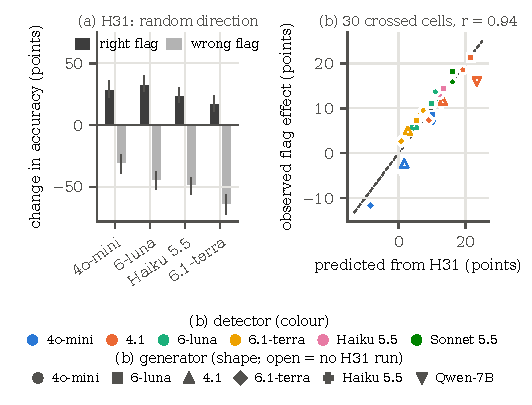
\includegraphics[width=\columnwidth]{generated/fig_reliability.pdf}
\caption{Left: randomised direction (H31; ConflictBank, one-answer prompt). Change in accuracy, with 95\% CIs, on
conflict questions given a right flag (naming the false side) or a wrong flag (naming the correct side). Right: the flag's effect in the \predAllN\ crossed detector--generator cells, predicted from H31's follow rates,
against the observed effect (filled: the generator's own follow rates; open: the mean follow rates, for generators
with no H31 run); dashed: $y=x$. Exploratory and retrospective: the account was defined after the cells were seen.
Table~\ref{tab:cells} lists the cells.}
\label{fig:reliability}
\end{figure}
\paragraph{A wrong flag costs more than a right one gains.} In a randomised test (H31), every ConflictBank conflict
question got a flag on its true contradiction, naming the false side on a random \nRandRight\ questions and the
correct side on the other \nRandWrong. A right flag raises accuracy by \hThirtyOneAMin\ to \hThirtyOneAMax\ points and
a wrong one lowers it by \ahThirtyOneBMax\ to \ahThirtyOneBMin\ (Figure~\ref{fig:reliability}, left). The net effect is
significantly negative for \nHThirtyOneCSig\ of \nHThirtyOneCTests\ generators at an even mix (H31c) and for
\nRealThirtyOneSig\ at the split as run (\shareRight\% right; gpt-6-luna \realThirtyOneLuna\ \realThirtyOneLunaCI).
For right- and wrong-flag effects $R$ and $W$, randomised flags on true pairs do net harm below a break-even
direction precision $p^\star=-W/(R-W)$: \beMini\ \beMiniCI\ for gpt-4o-mini, \beLuna\ for gpt-6-luna, \beHaiku\ for Claude
Haiku and \beTerra\ \beTerraCI\ for gpt-6.1-terra (Table~\ref{tab:breakeven}; exploratory). Right- and wrong-flag
follow rates overlap (descriptive; Table~\ref{tab:breakeven}) except gpt-6.1-terra's, so $p^\star$ rises mainly
because an accurate generator has more to lose. This threshold is a calibration: it carries over to a real detector only if
that detector flags typical questions and nothing else.

\paragraph{Real detectors are selective.} Across H24's \hTwentyFourCells\ detector--generator cells
(Table~\ref{tab:selection}), comparing precision with $p^\star$ can mislead. The gpt-4o-mini detector's precision
(\selHaikuMiniPrec\%) is just above Claude Haiku's break-even, implying \selHaikuMiniMarg\ points, but the cell's effect is
\selHaikuMiniObs: its flags on a correct passage (\selHaikuMiniWrongShare\% of questions) change accuracy there by
\selHaikuMiniWrongGain. The follow-rate account
$\hat\Delta=\frac1n\sum_i[d_i(1-a_i)f_R-w_ia_if_W]$ is a retrospective decomposition, defined after the cells were
seen, that uses each cell's coverage and no-flag accuracy ($d_i$: the flag
names the false side; $w_i$: it marks a correct passage; $a_i$: no-flag accuracy; $f_R,f_W$: H31's follow rates). The
account tracks the \predEightN\ cells with an H31 generator
($r=\predEightR$ \predEightRCI, mean error \predEightMae\ points, against \predGenMae\ for each generator's mean over
its other cells; $r=\predXfR$ with no-flag answers from another seed), mostly through the cell-level rates
(\predMargMae\ with cell means alone), but still misses the Haiku cell (\predHaikuMini). The registered H24 correlation is uninformative, since generator accuracy
enters both sides. The least precise detector (gpt-4o-mini, \dirPrecMini\%) lowers the accuracy of the four most
accurate generators, significantly for gpt-6.1-terra (H19).

\paragraph{What the detector contributes is its verdict.} The detector's judgement, passed as an answer key (``the
answer $X$ is false'' for the answer its suspect passage supports, no passage marked), matches the directional flag
(H30: \hThirtyAMin\ to \hThirtyAMax\ points per cell, none significant; pooled over the \PoolThirtyAK\ cells the flag
is ahead by \PoolThirtyA\ \PoolThirtyACI, equivalent within $\pm$3) and beats the detector model's own answer as a
hint by \PoolThirtyB\ \PoolThirtyBCI. That hint does worse than the flag in \nHTwentySevenAPos\ of
\nHTwentySevenATests\ cells and never better (H27).

\paragraph{With rare conflicts, false flags can outweigh gains.} The LLM detector also flags clean questions
(\cleanFprLlm\% of RAMDocs'). At a 5\% share of conflict questions its flag's estimate is negative in \prevNegFive\ of \prevN\ correlated settings
(bootstrap \prevNegFiveCI; significantly in \prevSigNeg, positive in \prevSigPos; Table~\ref{tab:prevalence}).

\paragraph{Genuine conflicts and baselines.} Reordering \citep{liu2024lost} or paraphrasing passages changes the
detectors' hit rate insignificantly (H29). Where both sides are valid, direction does damage (H28): on WikiContradict the LLM directional
flag lowers the share of answers giving both sides by \ahTwentyEightWcMiniDir\ to \ahTwentyEightWcLunaDir\ points
(and of answers correct under the benchmark's own rubric by \awikiOrigMiniEffPt\ to \awikiOrigLunaEffPt;
Appendix~\ref{app:semantic}). On RAMDocs' same-name questions, removal costs every generator
\ahTwentyEightAmbMiniRem\ to \ahTwentyEightAmbLunaRem\ points. Against published defences, with answer policies matched and TrustRAG's
system message restored, the LLM directional flag beats TrustRAG by \blHFourteenCbs\ points on ConflictBank and
\blHFourteenRd\ on RAMDocs, but not under majority misinformation (\blHFourteenMj). The registered H14, with
mismatched policies, shows no win (Appendix~\ref{app:extra}).
